% TraceLens paper — compile with pdflatex + bibtex
% Requires: acmart document class (tlmgr install acmart)

\documentclass[sigconf,nonacm]{acmart}

\usepackage[T1]{fontenc}
\usepackage{microtype}
\usepackage{tikz}
\usetikzlibrary{positioning, arrows.meta, calc}
% Styles for architecture TikZ figures (loaded from main.tex preamble)
\tikzset{
  archbox/.style={
    draw=black!55,
    rounded corners=2pt,
    align=center,
    font=\scriptsize,
    inner xsep=5pt,
    inner ysep=4pt,
  },
  % v2: blue = inputs/features, gray = pipeline, green = fusion core
  v2blue/.style={archbox, fill=blue!14, draw=blue!35, minimum width=19mm},
  v2gray/.style={archbox, fill=gray!12, draw=gray!45, minimum width=19mm},
  v2green/.style={archbox, fill=green!16, draw=green!40!black, minimum width=28mm},
  v2bus/.style={semithick, draw=black!65},
  v2arr/.style={-{Stealth[length=1.8mm, width=1.2mm]}, semithick, draw=black!65},
  v2legendbox/.style={
    draw=black!35,
    fill=white,
    rounded corners=2pt,
    inner xsep=8pt,
    inner ysep=5pt,
  },
  % v1
  v1gray/.style={archbox, fill=gray!12, draw=gray!45, minimum width=52mm},
  v1red/.style={archbox, fill=red!14, draw=red!45, minimum width=52mm},
  v1warn/.style={archbox, fill=yellow!20, draw=orange!50, minimum width=52mm},
  v1arr/.style={-{Stealth[length=1.8mm, width=1.2mm]}, semithick, draw=black!65},
}

% Colored swatch for legend tables (no nested tikz)
\newcommand{\archSwatch}[2]{%
  \raisebox{-0.35ex}{\fcolorbox{#1}{#2}{\rule{0pt}{2.6mm}\hspace{6.5mm}}}%
}

\newcommand{\vTwoLegendRow}{%
  \begin{tabular}{@{}c@{\hspace{1.5mm}}l@{\hspace{8mm}}c@{\hspace{1.5mm}}l@{\hspace{8mm}}c@{\hspace{1.5mm}}l@{}}%
    \archSwatch{blue!35}{blue!14} & {\scriptsize Inputs \& features} &
    \archSwatch{gray!45}{gray!12} & {\scriptsize Pipeline stages} &
    \archSwatch{green!40!black}{green!16} & {\scriptsize Fusion ranker} \\%
  \end{tabular}%
}

\newcommand{\vOneLegendRow}{%
  \begin{tabular}{@{}c@{\hspace{1.5mm}}l@{\hspace{8mm}}c@{\hspace{1.5mm}}l@{\hspace{8mm}}c@{\hspace{1.5mm}}l@{}}%
    \archSwatch{gray!45}{gray!12} & {\scriptsize Processing} &
    \archSwatch{red!45}{red!14} & {\scriptsize Rank override} &
    \archSwatch{orange!50}{yellow!20} & {\scriptsize Final output} \\%
  \end{tabular}%
}


\settopmatter{printacmref=false, printccs=true, printfolios=true}
\setcopyright{none}
\acmDOI{}
\acmISBN{}

\begin{document}

\title{TraceLens: Multimodal Relative Debugging of UI Test Regressions via Pass--Fail Trace Comparison}

\author{Musab Ahmed Khan}
\authornote{CS 460 Project, Sabanci University. Student ID: 33017.}
\affiliation{%
  \institution{Sabanci University}
  \city{Istanbul}
  \country{Turkey}
}
\email{musab.khan@sabanciuniv.edu}

\renewcommand{\shortauthors}{Musab Ahmed Khan}
% \renewcommand{\shorttitle}{TraceLens}

\begin{abstract}
When an automated UI test regresses from pass to fail, engineers practice \emph{relative debugging}: they compare two executions of the same test to find the earliest step whose divergence explains the failure, separating root cause from downstream symptoms.
We present \textsc{TraceLens}, a multimodal pipeline that aligns pass and fail traces, scores per-step \emph{relative anomalies} across network logs, console output, actions, navigation, and screenshots, and optionally reranks candidates with a large language model (LLM) and a vision-language model (VLM).
Our first architecture (v1) stacked heuristic ranking, LLM reranking, VLM ensemble, and trace-specific Hit@1 guards; hybrid mode proved brittle when guards tuned for one failure pattern regressed others.
We therefore introduce v2, which replaces post-hoc overrides with \emph{unified weighted fusion} and read-only diagnosis.
On a benchmark of 22 real UI regression traces, a heuristic baseline achieves 64\% Hit@1.
LLM-only reranking reaches \textbf{86\% Hit@1}, the best top-1 localization.
Hybrid LLM+VLM fusion reaches \textbf{82\% Hit@1} but \textbf{100\% Hit@3} with lower mean rank distance (0.27 vs.\ 0.32), recovering visually dominant cases while occasionally regressing when visual noise overrides causal text.
We recommend LLM-only for sharp top-1 localization and hybrid fusion when top-$k$ robustness and screenshot evidence matter.
\end{abstract}


\ccsdesc[500]{Software and its engineering~Software testing and debugging}
\ccsdesc[300]{Computing methodologies~Machine learning}

\keywords{relative debugging, regression diagnosis, UI testing, execution traces, fault localization, LLM, VLM}

\maketitle

% Running headers (sigconf twoside): short title (odd) / author (even),
% with CS 460 Project and Sabanci University on the opposite sides.
\makeatletter
\fancypagestyle{standardpagestyle}{%
  \fancyhf{}%
  \renewcommand{\headrulewidth}{\z@}%
  \renewcommand{\footrulewidth}{\z@}%
  \fancyfoot[C]{\if@ACM@printfolios\footnotesize\thepage\fi}%
  \fancyhead[LO]{\ACM@linecountL\@headfootfont\shorttitle}%
  \fancyhead[RO]{\ACM@linecountR\@headfootfont CS~460 Project}%
  \fancyhead[LE]{\ACM@linecountL\@headfootfont Sabanci University}%
  \fancyhead[RE]{\@headfootfont\@shortauthors\ACM@linecountR}%
}
\pagestyle{standardpagestyle}
\makeatother

%==============================================================================
\section{Introduction}
\label{sec:intro}

Automated end-to-end (E2E) UI tests produce rich \emph{execution traces}: ordered steps recording browser actions, HTTP traffic, console messages, and screenshots.
When a test that passed yesterday fails today, debugging is inherently \emph{relative}: engineers diff the good run against the bad run to locate where behavior first diverged.
We call this task \textbf{relative debugging}, following the compare-against-reference paradigm of Abramson et al.~\cite{abramson1996relative,sosic1997guard}: given a passing trace~$P$ and a failing trace~$F$ for the same test case, rank execution steps by how likely each is the \emph{earliest root cause} of the regression.

Relative debugging differs from classical source-level fault localization~\cite{wong2016survey,agrawal1995fault}.
The artifact under analysis is an \emph{execution trace}, not a program graph.
The supervision signal is the pass--fail \emph{pair} itself: anomalies are defined relative to what changed between runs.

Three difficulties recur in practice.
\textbf{(1)~Symptom vs.\ cause.}
A wrong credential at step~7 may surface only as a verification failure at step~8; ranking by error magnitude favors the symptom~\cite{panichella2015test}.
\textbf{(2)~Silent and visual faults.}
Missing form fields, CAPTCHA walls, and stale CDN assets may produce no console or network signal; only screenshots reveal the divergence~\cite{mesbah2012crawling}.
\textbf{(3)~Noise.}
Telemetry URLs, placeholder domains, and transient network flicker create spurious diffs that distract both heuristics and language models.

We built \textsc{TraceLens} to automate relative debugging for UI test traces.
The system parses heterogeneous trace formats, aligns pass and fail steps, extracts multimodal relative features, ranks suspicious steps, and generates technical and stakeholder-facing explanations.
We evaluate four modes against a \textbf{heuristic baseline} (pass--fail signal diffing without API calls): LLM reranking for causal text reasoning, VLM analysis for screenshot pairs, and hybrid fusion combining both.

\paragraph{Running example.}
On the \texttt{hackernews} trace, a Firebase timeout at step~12 causes many quiet steps afterward; heuristics rank a later verify step with higher pixel score.
The LLM reranker reads \texttt{errors\_observed\_on\_next\_step} and promotes step~12, a canonical \emph{relative} causal pattern.
On \texttt{amazon}, the ground-truth fault is an auth-gated click (step~20); LLM correctly places it first, but hybrid fusion elevates an earlier scroll step with large screenshot diff, illustrating the LLM/hybrid tradeoff we quantify in Section~\ref{sec:eval}.

Our evaluation on 22 traces shows complementary strengths rather than a single winner.
The heuristic baseline reaches 64\% Hit@1.
\textbf{LLM-only} mode achieves the highest Hit@1 (\textbf{86\%}), indicating strong text and causal ranking when logs and actions are informative.
\textbf{Hybrid} fusion matches or exceeds LLM on Hit@3 (100\% vs.\ 95\%) and on rank-quality metrics (lower mean rank distance and MAD@5), recovering visual-dominant or ambiguous cases (e.g., \texttt{github}) while occasionally regressing when visual noise overrides text (e.g., \texttt{amazon}).
We therefore treat LLM as the default for sharp top-1 localization and hybrid as the multimodal setting when top-$k$ robustness and visual evidence matter.

\paragraph{Contributions.}
\begin{itemize}
  \item \textbf{TraceLens}, an end-to-end relative debugging pipeline for UI regression traces with interpretable multimodal signals and stakeholder reports.
  \item \textbf{Multimodal relative features}, including navigation mismatch detection, visual-causal walk-back from persistent screenshot divergence, and observer vs.\ action attribution.
  \item \textbf{v2 unified fusion}, replacing v1's trace-specific guard stack with a single weighted ranker; LLM/VLM outputs are soft priors and diagnosis is read-only.
  \item \textbf{Empirical study} on 22 diverse traces with ablations and an LLM vs.\ hybrid tradeoff analysis.
\end{itemize}

%==============================================================================
\section{Background and Related Work}
\label{sec:related}

\paragraph{Relative and delta debugging.}
Abramson et al.~\cite{abramson1996relative} introduced \emph{relative debugging}: locating errors by comparing a suspect program's state against a trusted reference execution.
The \textsc{Guard} tool~\cite{sosic1997guard} operationalized this for scientific software evolution.
We adapt the same principle to UI test traces: the pass run is the reference and the fail run is the suspect; divergence is measured per aligned step rather than per variable.
Delta debugging~\cite{zeller2002simplifying} isolates failure-inducing \emph{inputs} by systematically simplifying test cases; relative debugging instead ranks \emph{execution steps} where pass and fail behavior diverge.
Trace comparison also appears in log analysis~\cite{grechanik2009recovering,panichella2015test} and web testing~\cite{ricca2001testing,mesbah2012crawling}, but prior tools rarely publish reproducible ranking metrics over multimodal UI traces with ground-truth fault steps.

\paragraph{Fault localization.}
Spectrum-based and learning-based fault localization~\cite{wen2020reproducing,wong2016survey} rank \emph{source entities} (statements, methods) using coverage and pass/fail test outcomes.
\textsc{TraceLens} instead ranks \emph{trace steps} using direct pass--fail diffs of actions, logs, and pixels.
The tasks are complementary: trace-step localization supports test maintainers; code-level FL supports developers patching production code.

\paragraph{LLMs and VLMs for software engineering.}
Recent surveys document LLM use for bug repair, log parsing, and code generation~\cite{kang2023llm,brown2020language}.
We use an LLM as a \emph{reranker} over compact relative features, not as a patch generator.
Vision-language models enable GUI understanding~\cite{deng2023webarena,liu2024mind2web,chen2024ui}; we apply VLMs to \emph{pass vs.\ fail screenshot pairs} at candidate steps identified by cheaper heuristics, controlling API cost.

\paragraph{Gap.}
No prior work combines (i)~heterogeneous real UI trace schemas, (ii)~explicit relative multimodal features, (iii)~LLM and VLM priors in one fusion ranker, and (iv)~Hit@$k$ evaluation including text-invisible faults, in a reproducible open-source implementation with frozen benchmark runs.

%==============================================================================
\section{Approach}
\label{sec:approach}

\begin{figure}[t]
  \centering
  \resizebox{\linewidth}{!}{%
    % TikZ v2 architecture — include inside \resizebox in main.tex
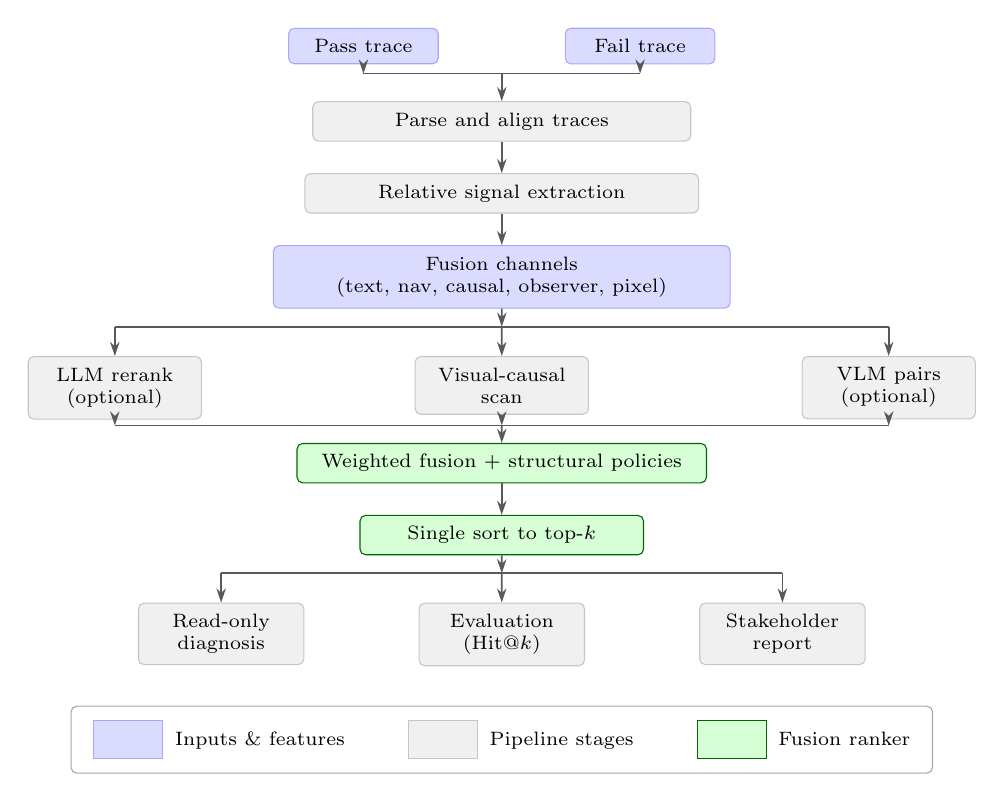
\begin{tikzpicture}[node distance=4mm]
  \node[v2blue] (pass) {Pass trace};
  \node[v2blue, right=16mm of pass] (fail) {Fail trace};

  \node[v2gray, below=7mm of $(pass)!0.5!(fail)$, minimum width=48mm] (parse)
    {Parse and align traces};
  \node[v2gray, below=of parse, minimum width=50mm] (signals)
    {Relative signal extraction};
  \node[v2blue, below=of signals, minimum width=58mm] (channels)
    {Fusion channels\\(text, nav, causal, observer, pixel)};

  \node[v2gray, below left=6mm and 9mm of channels, minimum width=22mm] (llm)
    {LLM rerank\\(optional)};
  \node[v2gray, below=6mm of channels, minimum width=22mm] (vc)
    {Visual-causal\\scan};
  \node[v2gray, below right=6mm and 9mm of channels, minimum width=22mm] (vlm)
    {VLM pairs\\(optional)};

  \node[v2green, below=7mm of $(llm)!0.5!(vlm)$, minimum width=52mm] (fusion)
    {Weighted fusion + structural policies};
  \node[v2green, below=of fusion, minimum width=36mm] (sort)
    {Single sort to top-$k$};

  \node[v2gray, below left=6mm and 7mm of sort, minimum width=21mm] (diag)
    {Read-only\\diagnosis};
  \node[v2gray, below=6mm of sort, minimum width=21mm] (eval)
    {Evaluation\\(Hit@$k$)};
  \node[v2gray, below right=6mm and 7mm of sort, minimum width=21mm] (report)
    {Stakeholder\\report};

  % --- arrows ---
  \coordinate (inBus) at ($(parse.north) + (0,3.5mm)$);
  \draw[v2bus] (pass.south |- inBus) -- (fail.south |- inBus);
  \draw[v2arr] (pass.south) -- (pass.south |- inBus);
  \draw[v2arr] (fail.south) -- (fail.south |- inBus);
  \draw[v2arr] (inBus) -- (parse.north);

  \draw[v2arr] (parse.south) -- (signals.north);
  \draw[v2arr] (signals.south) -- (channels.north);

  \coordinate (splitBus) at ($(channels.south)!0.38!(vc.north)$);
  \draw[v2bus] (splitBus -| llm.north) -- (splitBus -| vlm.north);
  \draw[v2arr] (channels.south) -- (splitBus);
  \draw[v2arr] (splitBus -| llm.north) -- (llm.north);
  \draw[v2arr] (splitBus) -- (vc.north);
  \draw[v2arr] (splitBus -| vlm.north) -- (vlm.north);

  \coordinate (joinBus) at ($(vc.south)!0.38!(fusion.north)$);
  \draw[v2bus] (joinBus -| llm.south) -- (joinBus -| vlm.south);
  \draw[v2arr] (llm.south) -- (joinBus -| llm.south);
  \draw[v2arr] (vc.south) -- (joinBus);
  \draw[v2arr] (vlm.south) -- (joinBus -| vlm.south);
  \draw[v2arr] (joinBus) -- (fusion.north);

  \draw[v2arr] (fusion.south) -- (sort.north);

  \coordinate (outBus) at ($(sort.south)!0.38!(eval.north)$);
  \draw[v2bus] (outBus -| diag.north) -- (outBus -| report.north);
  \draw[v2arr] (sort.south) -- (outBus);
  \draw[v2arr] (outBus -| diag.north) -- (diag.north);
  \draw[v2arr] (outBus) -- (eval.north);
  \draw[v2arr] (outBus -| report.north) -- (report.north);

  % --- legend: one row, centered, boxed ---
  \node[v2legendbox, anchor=north, below=5mm of eval.south] {\vTwoLegendRow};
\end{tikzpicture}
%
  }
  \caption{\textsc{TraceLens} v2 pipeline. Pass and fail traces are parsed, aligned, and differenced into fusion channels; optional LLM/VLM priors feed a single weighted sort. Diagnosis is read-only.}
  \Description{Flowchart of the v2 pipeline from pass/fail traces through fusion to ranked output.}
  \label{fig:arch-v2}
\end{figure}

Figure~\ref{fig:arch-v2} summarizes our v2 architecture (entry point \texttt{main2.py}).
Section~\ref{sec:v1} briefly describes v1, which we supersede.

\subsection{Task formulation}
\label{sec:task}

\textbf{Input:} passing trace $P = (p_0,\ldots,p_{n-1})$ and failing trace $F = (f_0,\ldots,f_{m-1})$ for the same test.

\textbf{Output:} ranked step list $(s_1,\ldots,s_k)$, a technical diagnosis, and a plain-language summary.

Each step is unified into a schema with action text, action type, optional intent field (one data source), network logs, console logs, and screenshot path.
Alignment uses index-based pairing when $|P|=|F|$; otherwise action-similarity alignment when faults insert or delete steps.

Ground truth is a single fault step index per trace (used only for evaluation).
Metrics: Hit@$k$ (GT in top-$k$), mean rank distance $|\mathrm{rank}(GT) - 1|$, and MAD@5 (mean absolute deviation of GT rank from~1, capped at~5).

\subsection{Relative signal extraction (heuristic baseline)}
\label{sec:heuristic}

The \textbf{heuristic baseline} scores each aligned pair $(p_i, f_i)$ without API calls.
Four text signals in $[0,1]$ are combined with fixed weights (renormalized when intent is absent):

\begin{itemize}
  \item \textbf{Network:} new HTTP errors, status changes, or missing expected requests in~$F$.
  \item \textbf{Console:} new JavaScript errors or warnings in~$F$.
  \item \textbf{Action:} divergence in action text or type between~$P$ and~$F$.
  \item \textbf{Intent:} changed verification outcome strings (available on one source schema).
\end{itemize}

\textbf{Navigation signals} detect wrong-page loads: expected URL absent and unintended page present (\texttt{wrong\_navigation}), boosting steps that explain silent navigation faults.

\textbf{Noise filtering} removes placeholder domains (e.g., \texttt{example.com} distractors) and known telemetry patterns so relative diffs focus on test-relevant traffic.

\textbf{Pixel diff} (local, no API) compares pass/fail PNGs for the heuristic top-5; enabled by default, disabled with \texttt{--no-pixel}.

Table~\ref{tab:signals} summarizes signals; the baseline mode is \texttt{python main2.py} without flags.

\begin{table}[t]
  \caption{Pass--fail relative signals in \textsc{TraceLens}.}
  \label{tab:signals}
  \small
  \begin{tabular}{p{0.18\linewidth}p{0.38\linewidth}p{0.28\linewidth}}
    \toprule
    Signal & Relative comparison & Example \\
    \midrule
    Network & New/changed errors in fail & HTTP 500 \\
    Console & New JS errors in fail & UI crash \\
    Action & Text or type diverges & Invalid form \\
    Navigation & Wrong page loaded & Wrong click \\
    Pixel & Screenshot diff & Visual regression \\
    \bottomrule
  \end{tabular}
\end{table}

\subsection{Visual relative signals}
\label{sec:visual}

Three visual layers differ in scope and cost:

\textbf{Pixel boost} computes mean pixel difference on aligned PNG pairs (local, cheap).

\textbf{Visual-causal attribution} scans all steps when visual mode is enabled, finds the earliest \emph{persistent} screenshot divergence, and walks back to a silent cause step (e.g., missing zipcode visible only on the next screen).
This uses deterministic rules, not a neural model.

\textbf{VLM analysis} sends pass/fail pairs for top-$K$ candidates (${\sim}5$ steps) to a vision-language model, returning per-step visual scores and a suggested root step.
Visual-causal steps are injected into the VLM candidate pool; scores can backfill from symptom steps onto cause steps.

\subsection{LLM relative reranking}
\label{sec:llm}

With \texttt{--llm}, a language model reranks a candidate pool: heuristic top-15 plus injected steps with strong navigation, causal, or action-changed signals.
The prompt exposes compact \emph{relative} fields (\texttt{action\_changed}, \texttt{wrong\_navigation}, filtered network/console snippets) without screenshots.

The LLM returns an ordered list and a diagnosis.
In \textbf{v2}, rerank positions map to an \texttt{llm\_prior} fusion channel; diagnosis \textbf{does not} change the final rank.

We use OpenRouter with temperature~$0.0$ (Nemotron-3-Super-120B for text) to maximize reproducibility; provider routing may still introduce variance.

\subsection{v2 unified fusion}
\label{sec:fusion}

v2's main design contribution is a \textbf{single fusion score} per step:
\begin{equation}
  S(i) = \sum_{c \in \mathcal{C}} w_c \cdot f_c(i)
\end{equation}
where channels $\mathcal{C}$ include text, navigation, causal action, observer symptom, visual causal, pixel, and optionally LLM and VLM priors (denoted \texttt{llm\_prior} and \texttt{vlm\_prior} in code).
Weights $w_c$ are fixed in configuration (\texttt{llm\_prior}${}=0.28$, \texttt{vlm\_prior}${}=0.18$, mirroring v1's 60/40 LLM/VLM blend).

\textbf{Causal attribution} distinguishes \emph{action} steps (clicks, typing) from \emph{observer} steps (verify, wait).
When errors appear on a verify step, a preceding action step may be the true relative root (\texttt{causal\_action} channel).
When the verify step itself is labeled as ground truth (symptom-on-verify faults), observer channels must not be over-capped; v1 learned this through per-trace guards, v2 encodes it as channel weights and the observer-after-causal cap.

\textbf{Structural policies} (not trace-specific guards) adjust scores:
\begin{itemize}
  \item \textbf{Observer cap:} limit verify-step visual weight when a prior causal action step has strong text support.
  \item \textbf{Downstream penalty:} demote steps after inferred root, with exemption when text signal exceeds a threshold.
  \item \textbf{LLM/action bonuses:} small nudges when the LLM ranks a causal or action-changed step first.
\end{itemize}

Steps are sorted once by~$S(i)$.
Hybrid mode (\texttt{--llm --vlm}) activates all channels; LLM-only and VLM-only use the same scorer with different channel subsets.

\paragraph{Mode summary.}
\begin{itemize}
  \item \textbf{Heuristic (baseline):} fast, interpretable pass--fail diff; 64\% Hit@1; misses causal reasoning on hard traces.
  \item \textbf{LLM:} best Hit@1 (86\%); strong when logs and actions encode causality.
  \item \textbf{VLM:} addresses visual faults; weaker alone on network-heavy traces; higher latency and cost.
  \item \textbf{Hybrid:} best Hit@3 and rank distance; trades one Hit@1 vs.\ LLM when visual channel overweighted.
\end{itemize}

\subsection{v1 architecture and limitations}
\label{sec:v1}

\begin{figure}[t]
  \centering
  \resizebox{0.92\linewidth}{!}{%
    % TikZ v1 architecture — include inside \resizebox in main.tex
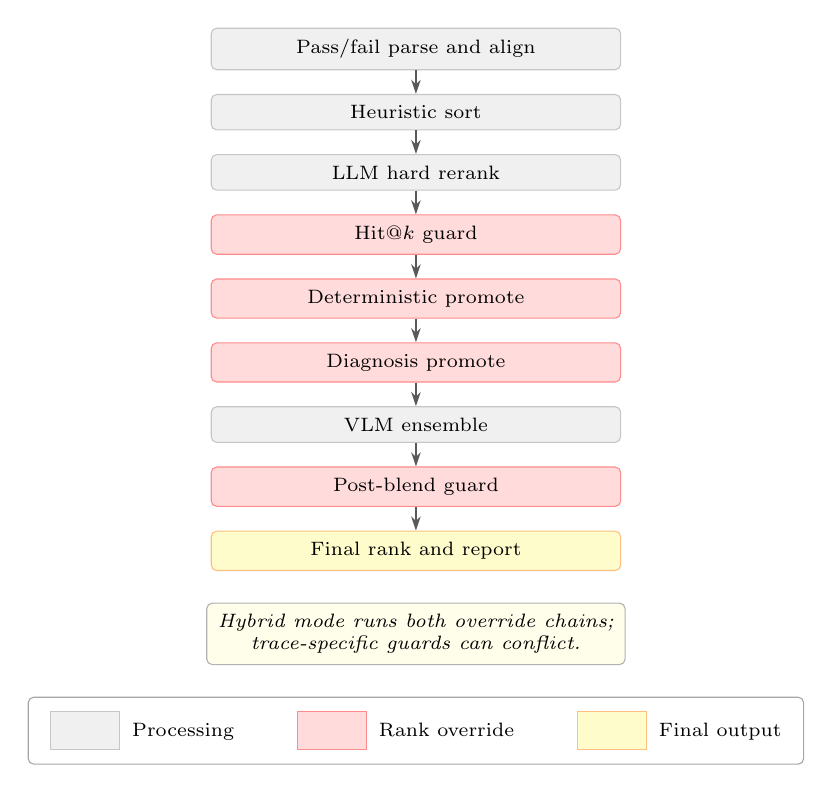
\begin{tikzpicture}[node distance=3mm]
  \node[v1gray] (s1) {Pass/fail parse and align};
  \node[v1gray, below=of s1] (s2) {Heuristic sort};
  \node[v1gray, below=of s2] (s3) {LLM hard rerank};
  \node[v1red, below=of s3] (s4) {Hit@$k$ guard};
  \node[v1red, below=of s4] (s5) {Deterministic promote};
  \node[v1red, below=of s5] (s6) {Diagnosis promote};
  \node[v1gray, below=of s6] (s7) {VLM ensemble};
  \node[v1red, below=of s7] (s8) {Post-blend guard};
  \node[v1warn, below=of s8] (s9) {Final rank and report};

  \foreach \a/\b in {s1/s2, s2/s3, s3/s4, s4/s5, s5/s6, s6/s7, s7/s8, s8/s9} {
    \draw[v1arr] (\a.south) -- (\b.north);
  }

  \node[font=\scriptsize\itshape, align=center, below=4mm of s9,
        draw=black!30, fill=yellow!8, rounded corners=2pt, inner sep=4pt] (note) {%
    Hybrid mode runs both override chains;\\
    trace-specific guards can conflict.};

  \node[v2legendbox, anchor=north, below=4mm of note.south] {\vOneLegendRow};
\end{tikzpicture}
%
  }
  \caption{v1 stacked pipeline (\texttt{main.py}). Highlighted stages can override prior rankings. Hybrid runs LLM overrides before VLM overrides and a second guard pass.}
  \Description{Vertical flowchart of the v1 pipeline with override stages marked.}
  \label{fig:arch-v1}
\end{figure}

Figure~\ref{fig:arch-v1} shows v1 (\texttt{main.py}), our first production architecture.
It validated that relative text and visual evidence are both necessary, but ranking policy was \textbf{fragmented}:
heuristic sort, then LLM hard rerank, Hit@1 guard, deterministic promote, diagnosis promote, VLM ensemble, and post-blend guard.

Guards encoded patterns from individual benchmark traces (promote causal action on \texttt{hackernews}; lock strong verify-pixel on \texttt{youtube}; suppress spurious scroll on \texttt{amazon}).
Tuning for one pattern regressed others; e.g., blocking deterministic promotes under visual lock sharply dropped accuracy on action-labeled traces in an intermediate experiment.

Hybrid mode (\texttt{--llm --vlm}) activated both override chains, so conflicts surfaced more often than in single-modality modes.
On partial benchmark runs, v1 hybrid underperformed LLM-only despite each modality working well in isolation.
Diagnosis and deterministic rules could also promote steps to rank~1 using patterns discovered while inspecting labeled traces, complicating claims of a general ranking policy.

\textbf{v2 response:} one fusion function, soft LLM/VLM priors, read-only diagnosis, structural caps replacing per-trace guard exceptions.
v1 remains in the repository as a reference implementation; all reported main results use v2.

%==============================================================================
\section{Evaluation}
\label{sec:eval}

\subsection{Research questions}

\textbf{RQ1:} How much do LLM and multimodal fusion improve relative step ranking over the heuristic baseline?

\textbf{RQ2:} What is the contribution of pixel/visual channels?

\textbf{RQ3:} How do LLM-only and hybrid compare on Hit@1 vs.\ top-$k$ and rank-quality metrics?

\textbf{RQ4:} How does performance vary across data sources and fault signal types?

\subsection{Benchmark and setup}

We evaluate on \textbf{22 traces} from three independent collections: 8 from efe/irem, 10 from areeb/salem, and 4 from ersel (reported as a \emph{test set} in figures due to distinct schema and intent fields).
Ground truth specifies one fault step per trace.
Table~\ref{tab:benchmark} summarizes fault-type frequencies; the full trace catalog is in our repository.

\begin{table}[t]
  \caption{Benchmark fault-type frequencies ($n{=}22$ traces). Coverage is collector-driven (e.g., seven HTTP-error traces, one JS exception).}
  \label{tab:benchmark}
  \small
  \begin{tabular}{lr}
    \toprule
    Failure type & $n$ \\
    \midrule
    HTTP 404/500 & 7 \\
    Wrong navigation / invalid input & 5 \\
    UI state mismatch & 3 \\
    Timeout / connection lost & 2 \\
    Auth-gated / credential failure & 2 \\
    Backend OK, frontend fail & 2 \\
    JS exception & 1 \\
    \bottomrule
  \end{tabular}
\end{table}

All main results use v2 (\texttt{main2.py}) with frozen run JSONs listed in \texttt{scripts/metrics\_manifest.yaml}.
Baseline: \texttt{python main2.py}.
\textbf{Models (free tier).}
LLM: \texttt{nvidia/nemotron-3-super-120b-a12b:free} via OpenRouter ($T{=}0$).
VLM: \texttt{meta-llama/llama-4-scout-17b-16e-instruct} via Groq ($T{=}0$), ${\sim}5$ screenshot pairs per trace.
We chose separate free-tier providers to stay within daily quotas without paid credits; this constrains model choice and throughput relative to commercial APIs.

\subsection{Results}

Table~\ref{tab:main} reports aggregate v2 metrics on all 22 traces.

\begin{table}[t]
  \caption{v2 aggregate results on 22 traces. Baseline = heuristic with pixel. VLM $n{=}21$ (\texttt{dictionary} excluded: incomplete screenshot pairs for top-$K$ candidates).}
  \label{tab:main}
  \small
  \begin{tabular}{lrrrrr}
    \toprule
    Mode & $n$ & Hit@1 & Hit@3 & Hit@5 & MRD \\
    \midrule
    Heuristic & 22 & 64\% & 91\% & 91\% & 0.86 \\
    No pixel & 22 & 68\% & 86\% & 91\% & 0.86 \\
    LLM & 22 & \textbf{86\%} & 95\% & 100\% & 0.32 \\
    VLM & 21 & 67\% & 95\% & 100\% & 0.43 \\
    Hybrid & 22 & 82\% & \textbf{100\%} & 100\% & \textbf{0.27} \\
    \bottomrule
  \end{tabular}

  \vspace{4pt}
  {\footnotesize MRD = mean rank distance. MAD@5: Heuristic 7.94, LLM 6.94, Hybrid 6.07.}
\end{table}

\textbf{RQ1.} LLM improves Hit@1 from 64\% to 86\% (+22 points); hybrid reaches 82\% (+18).
Every mode except no-pixel heuristic beats the baseline on Hit@3 or rank distance.

\textbf{RQ2.} Removing pixel changes Hit@1 from 64\% to 68\% on this corpus; marginal on aggregate, but pixel and visual-causal channels are essential for screenshot-primary faults (Section~\ref{sec:case}).

\textbf{RQ3.} Figure~\ref{fig:tradeoff} summarizes the LLM vs.\ hybrid tradeoff.
Hybrid wins Hit@3 (100\% vs.\ 95\%) and mean rank distance (0.27 vs.\ 0.32) but loses one Hit@1 (18/22 vs.\ 19/22).

\begin{figure}[t]
  \centering
  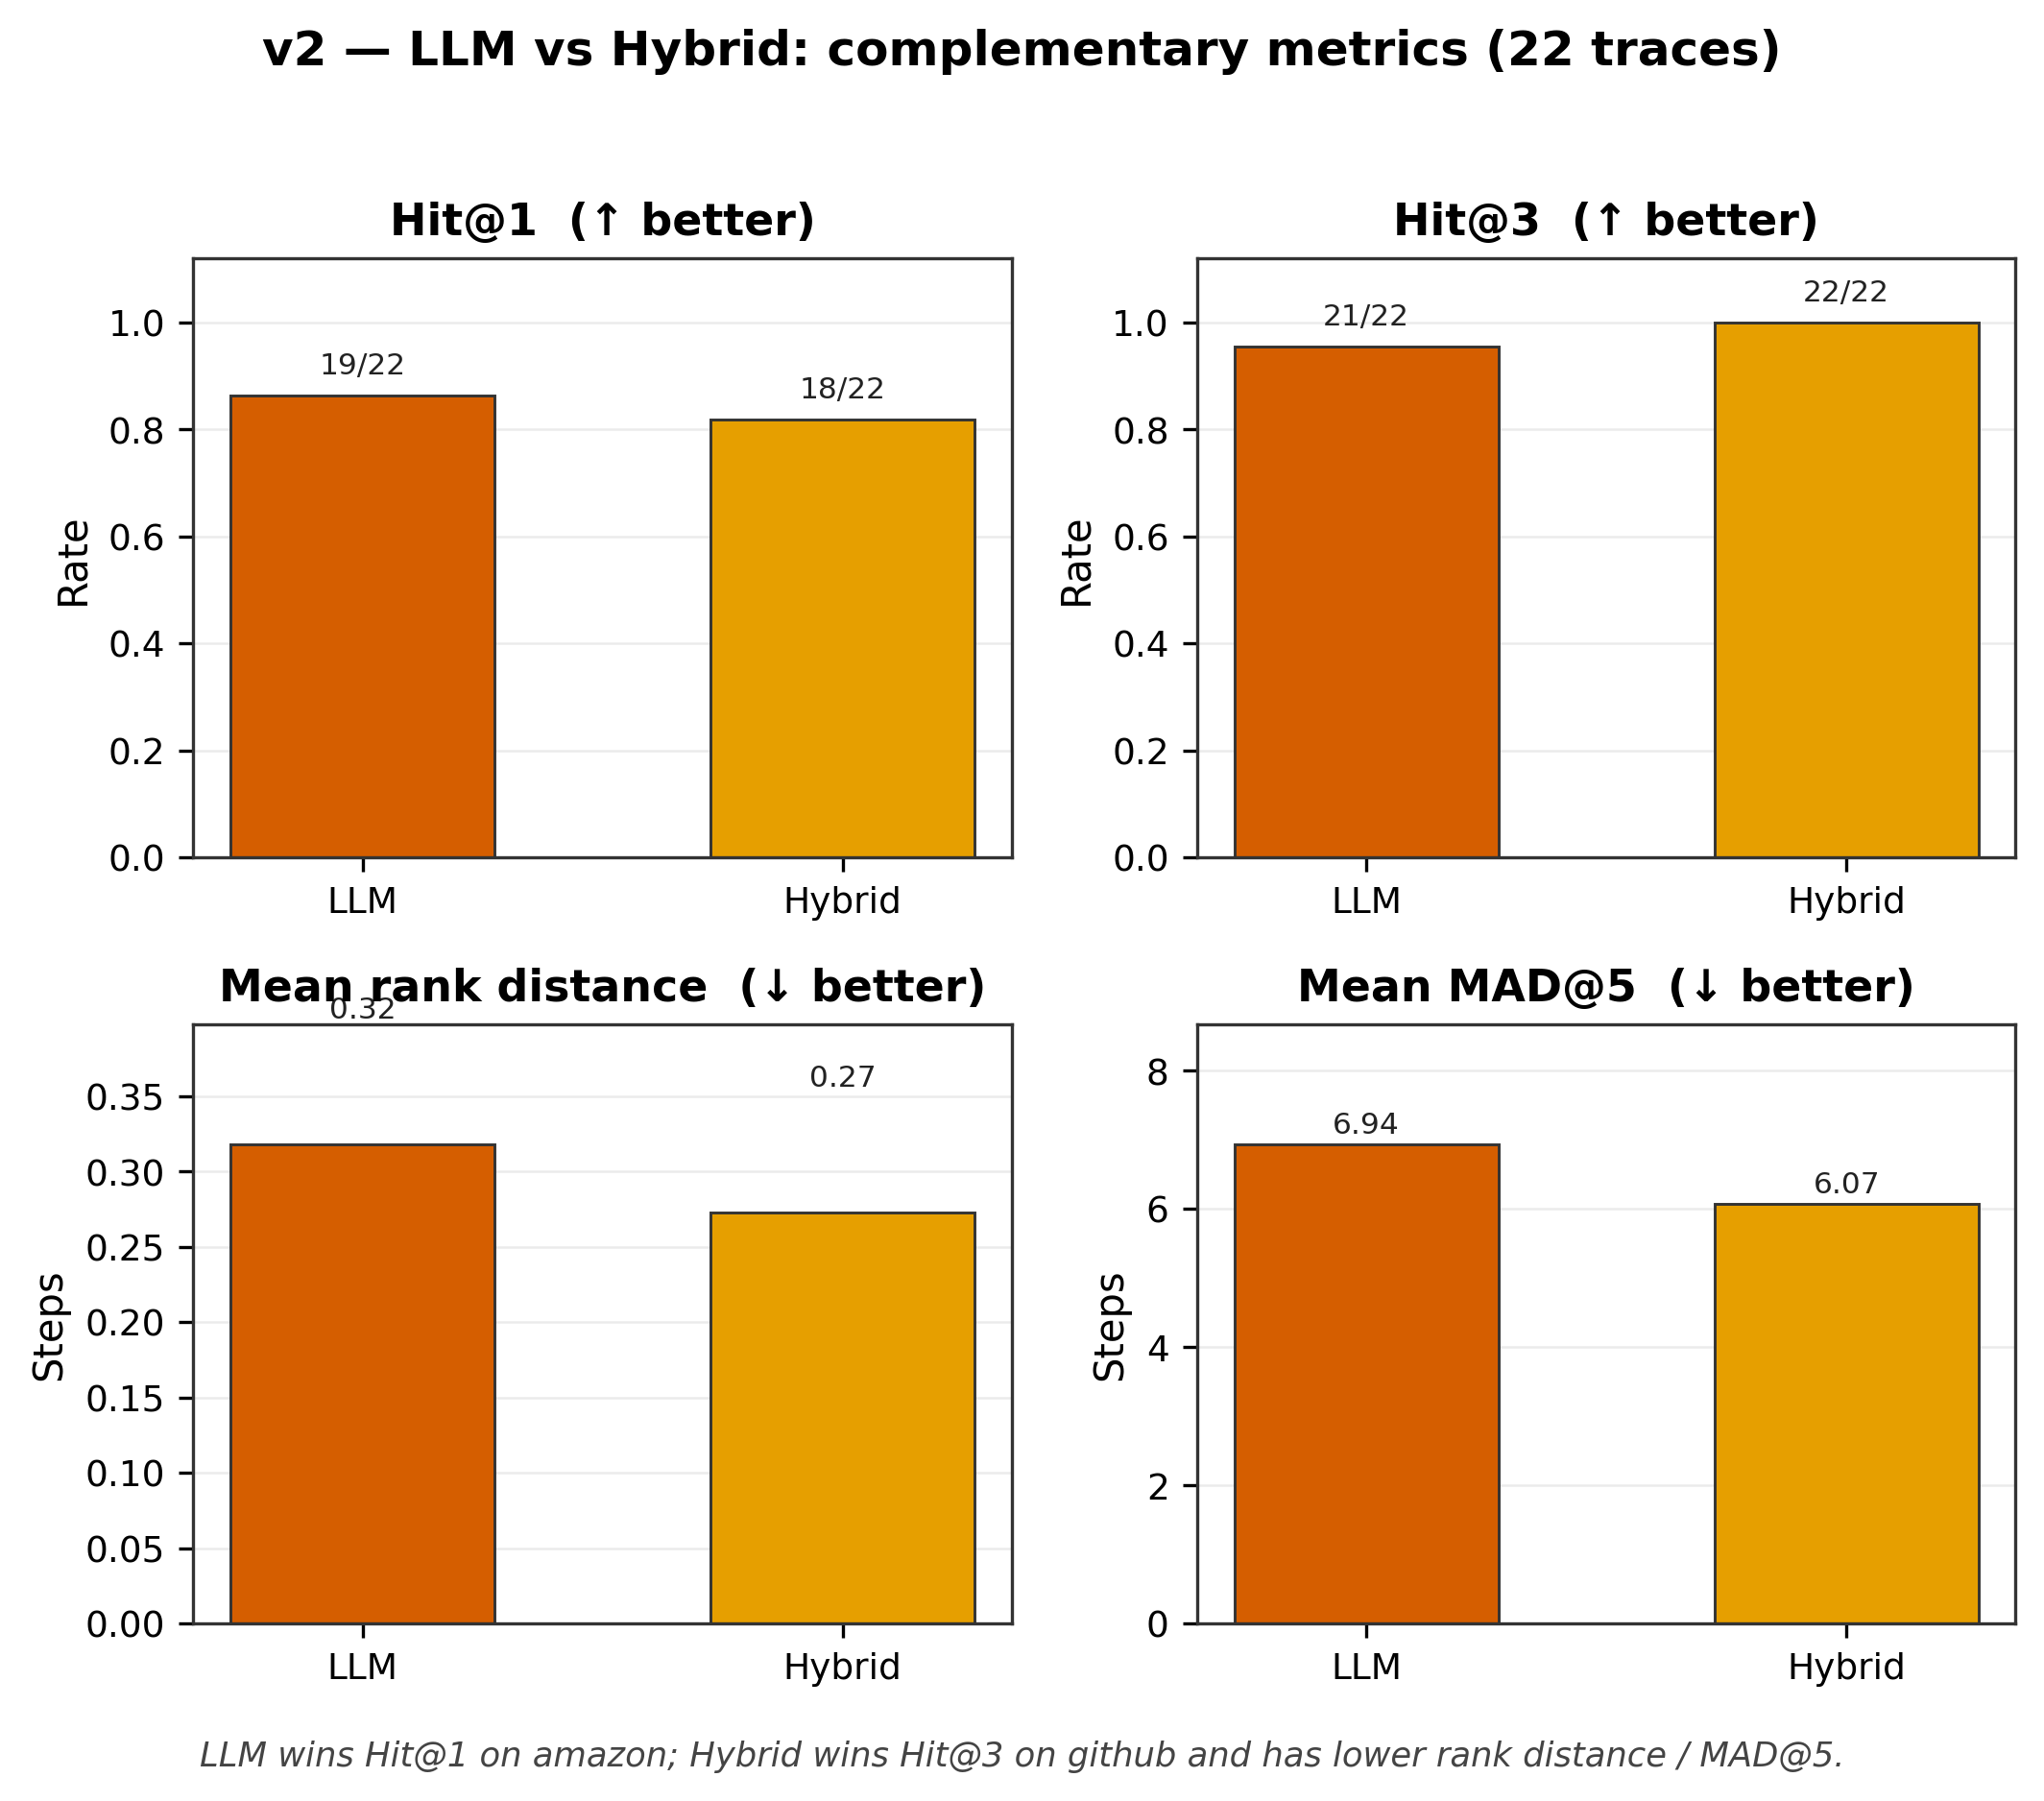
\includegraphics[width=\linewidth]{figures/fig6_llm_vs_hybrid_tradeoff.png}
  \caption{LLM vs.\ hybrid on Hit@1/3, mean rank distance, and MAD@5 (v2, 22 traces).}
  \Description{Bar chart comparing LLM and hybrid metrics.}
  \label{fig:tradeoff}
\end{figure}

\begin{figure}[t]
  \centering
  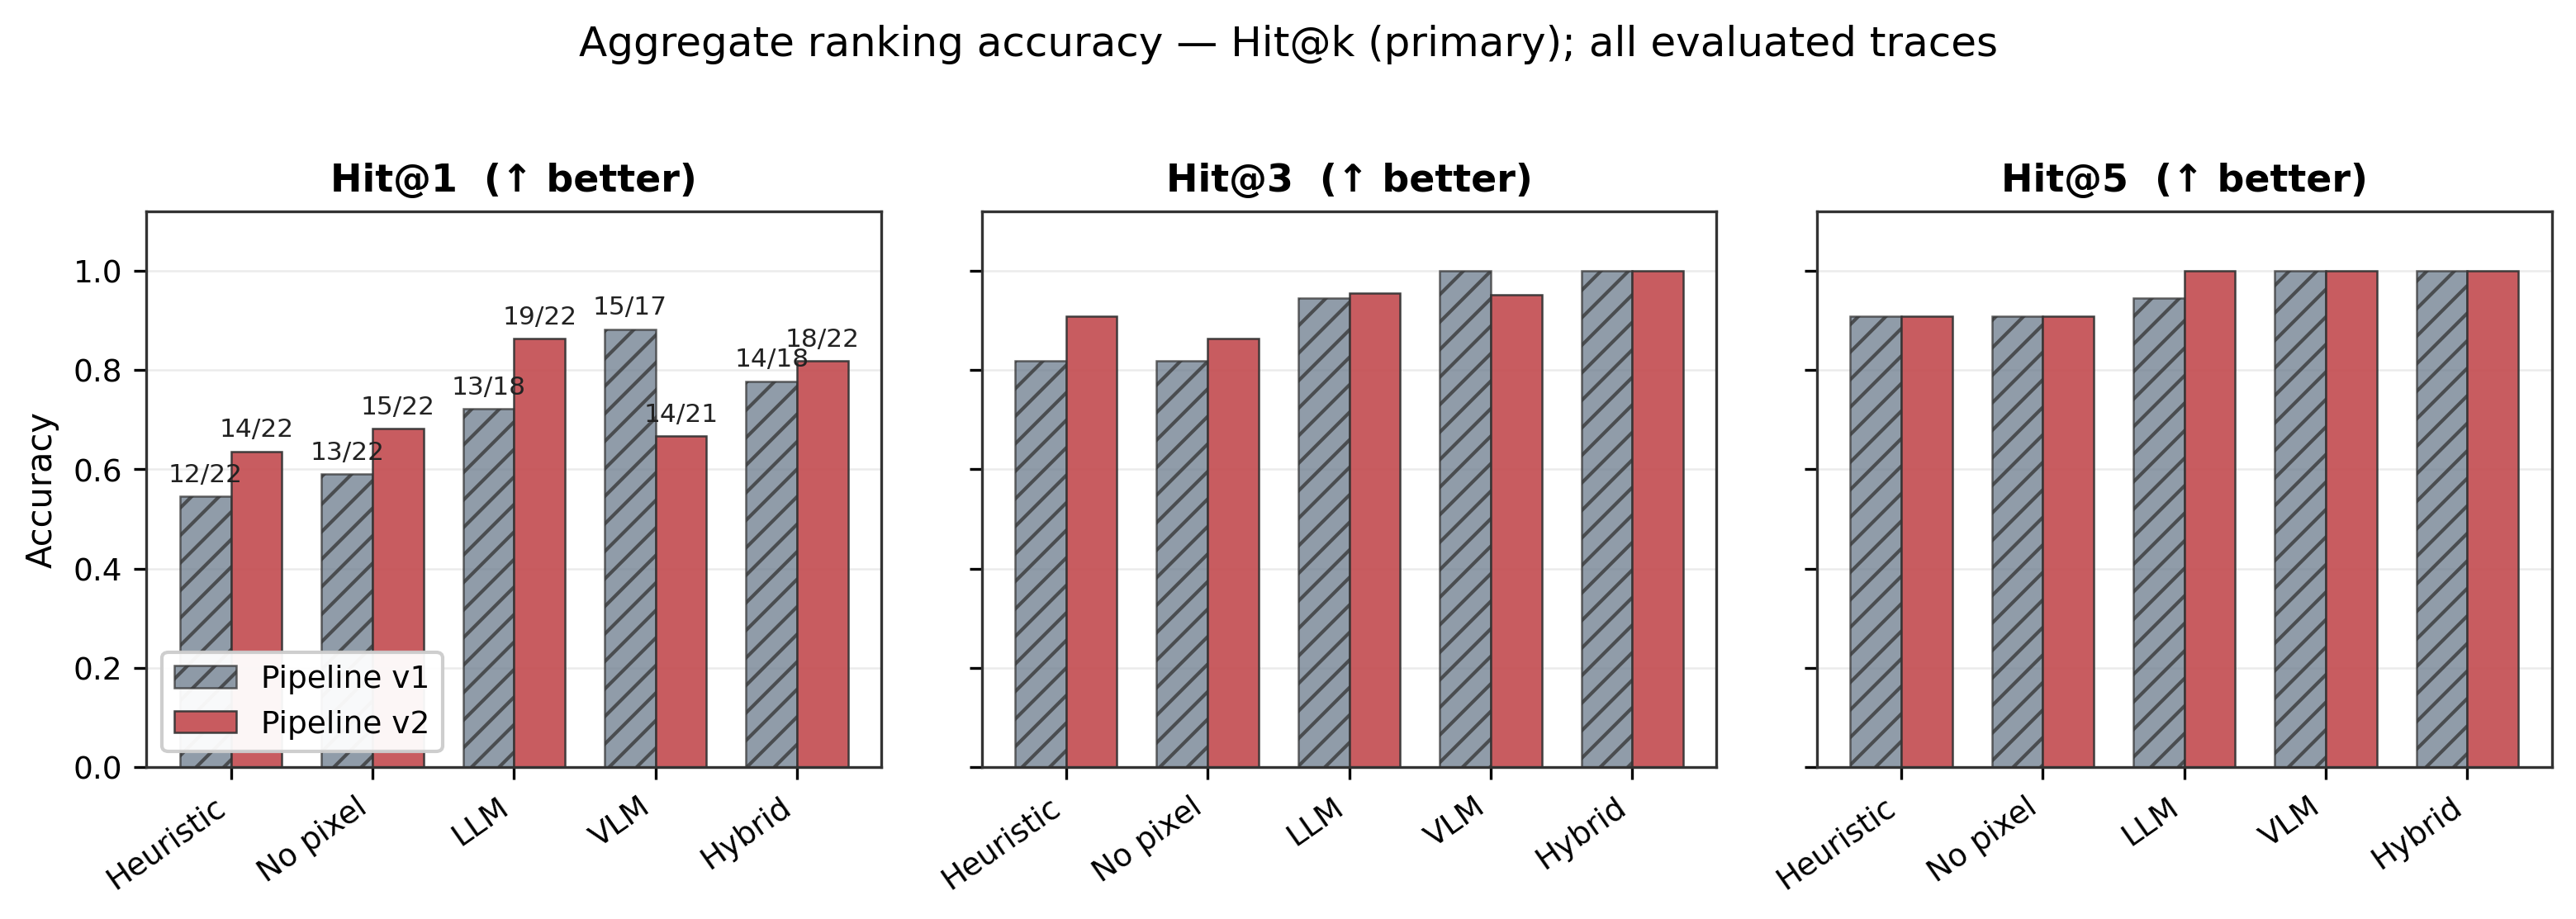
\includegraphics[width=\linewidth]{figures/fig1_aggregate_hitk.png}
  \caption{Hit@1/3/5 across modes; v1 vs.\ v2 evolution. Heuristic is the baseline.}
  \Description{Grouped bar chart of Hit@k for all pipeline modes.}
  \label{fig:hitk}
\end{figure}

\begin{figure}[t]
  \centering
  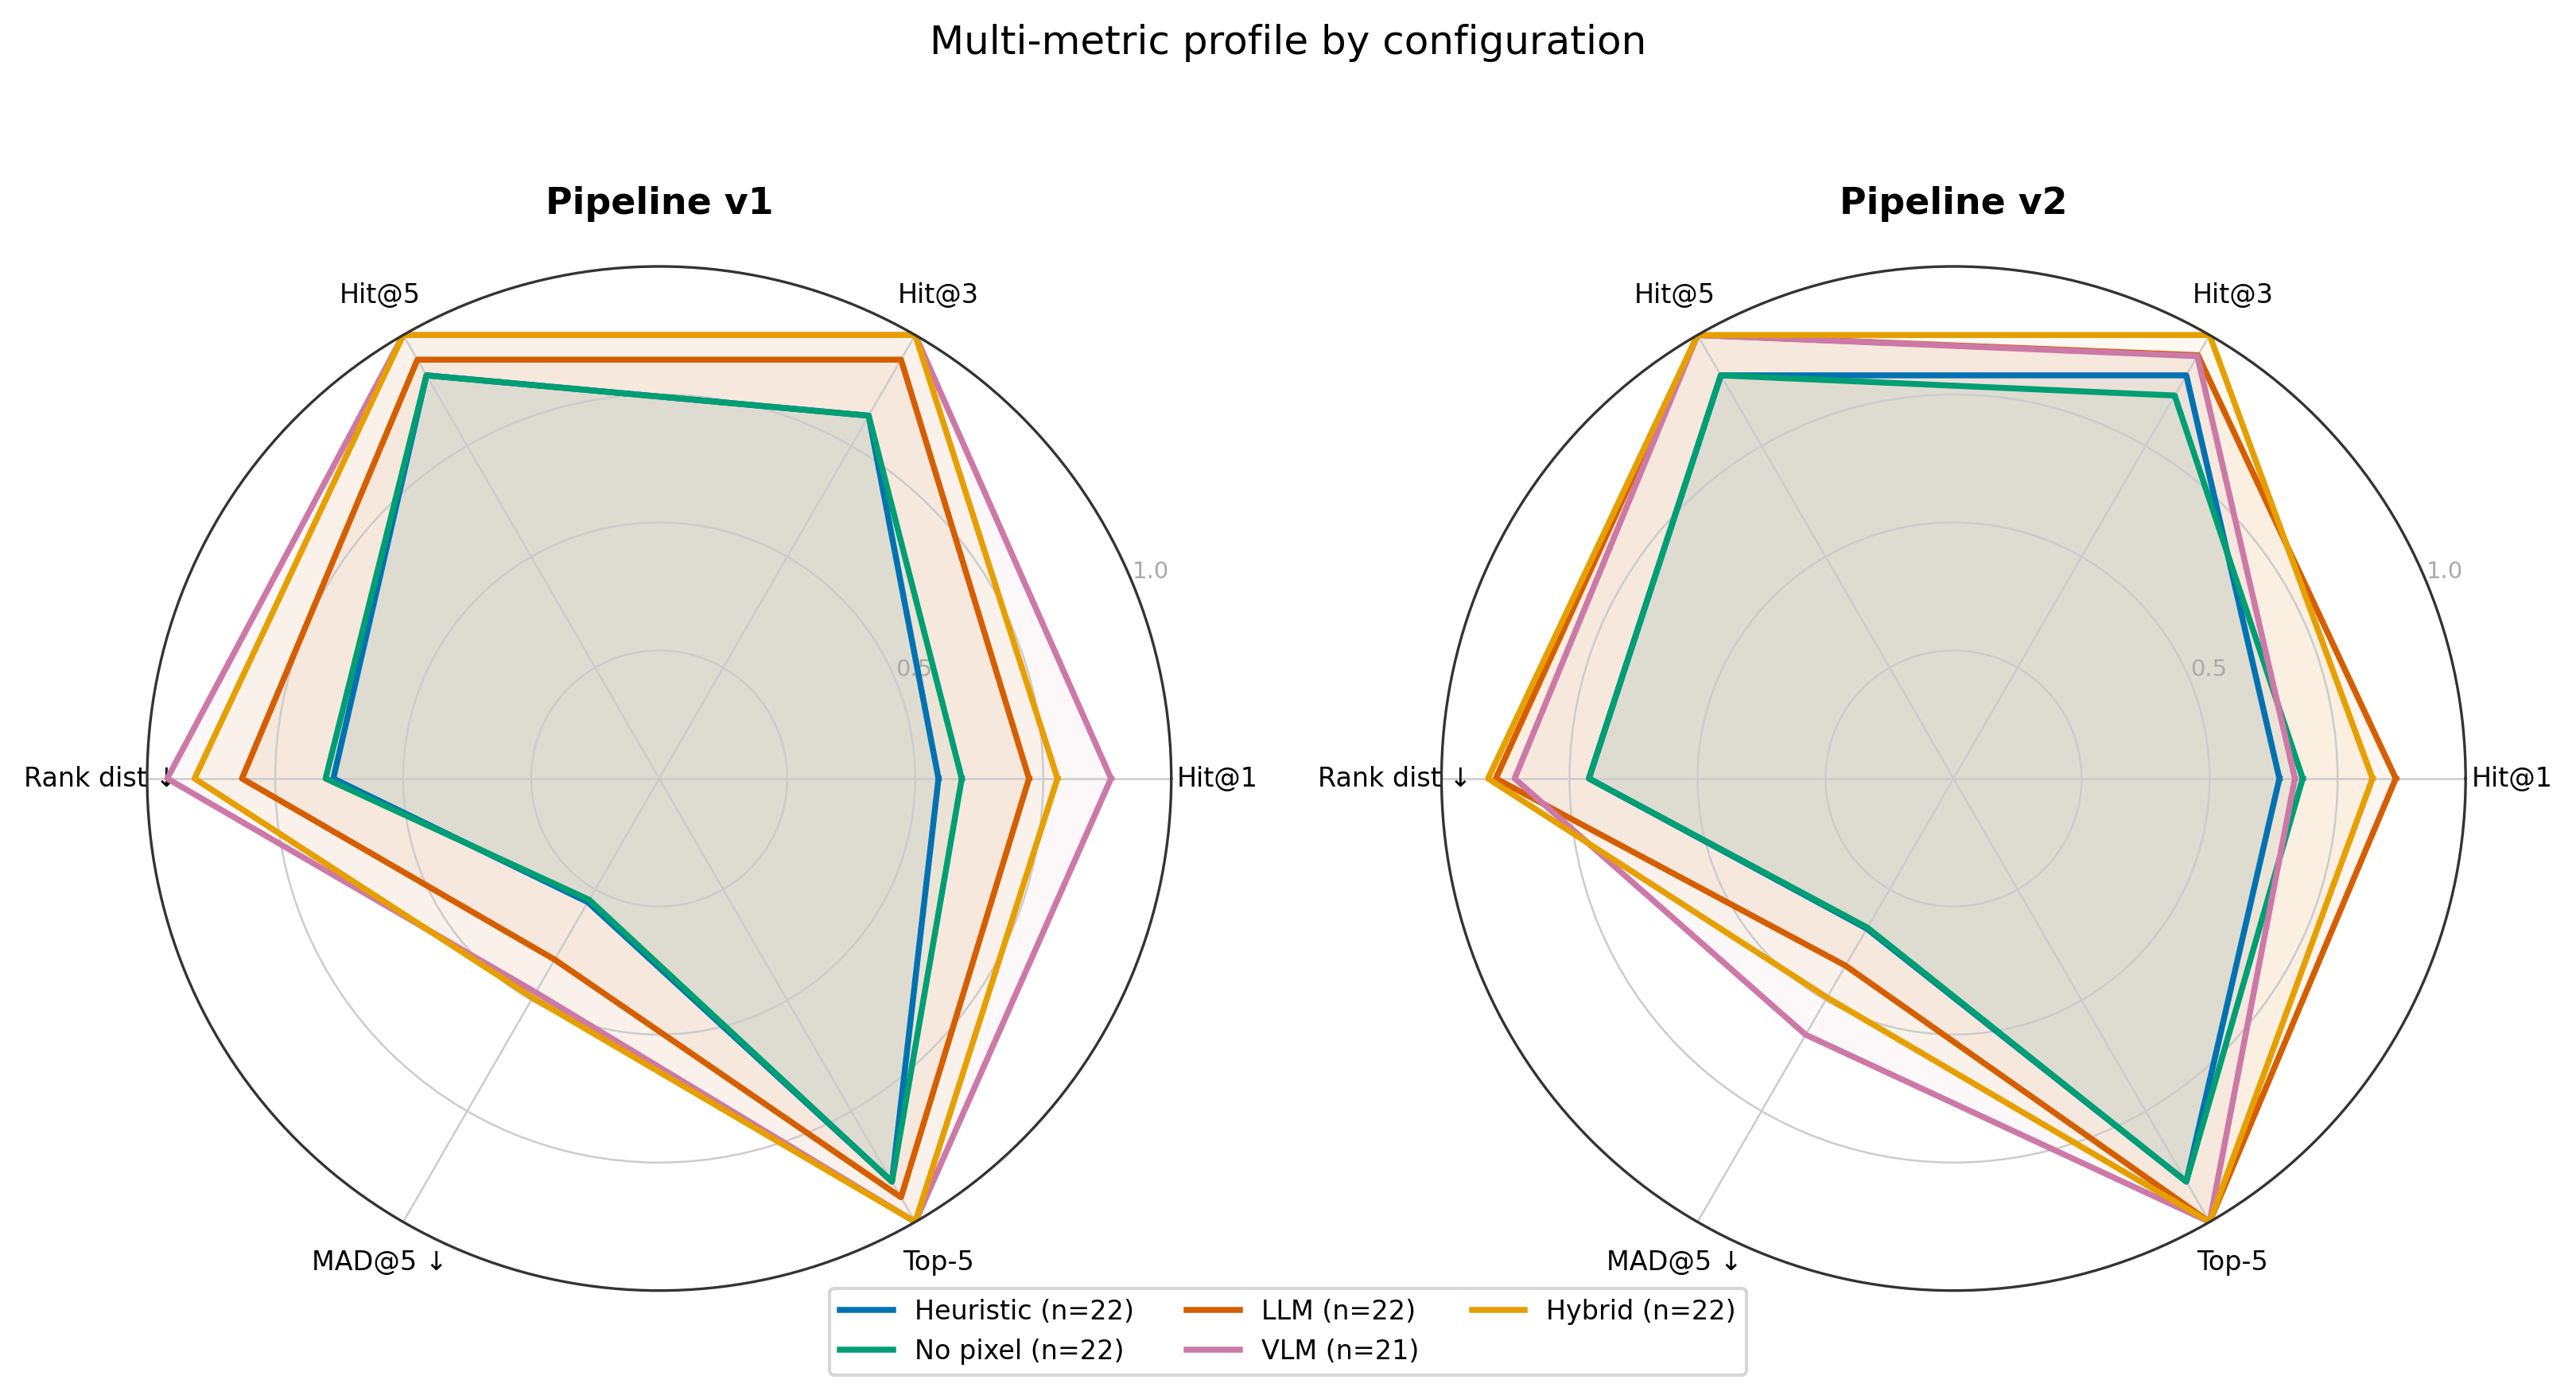
\includegraphics[width=\linewidth]{figures/fig5_radar_combined.png}
  \caption{Multi-metric radar comparison across v1 and v2 modes (Hit@1/3/5, rank distance, MAD@5).}
  \Description{Radar chart comparing aggregate metrics for v1 and v2 configurations.}
  \label{fig:radar}
\end{figure}

Figure~\ref{fig:hitk} shows Hit@$k$ across all modes; Figure~\ref{fig:radar} summarizes multiple metrics on a common scale.
Figure~\ref{fig:heatmap} gives per-trace Hit@1; Figure~\ref{fig:source} breaks Hit@1 by source collection.

\begin{figure}[t]
  \centering
  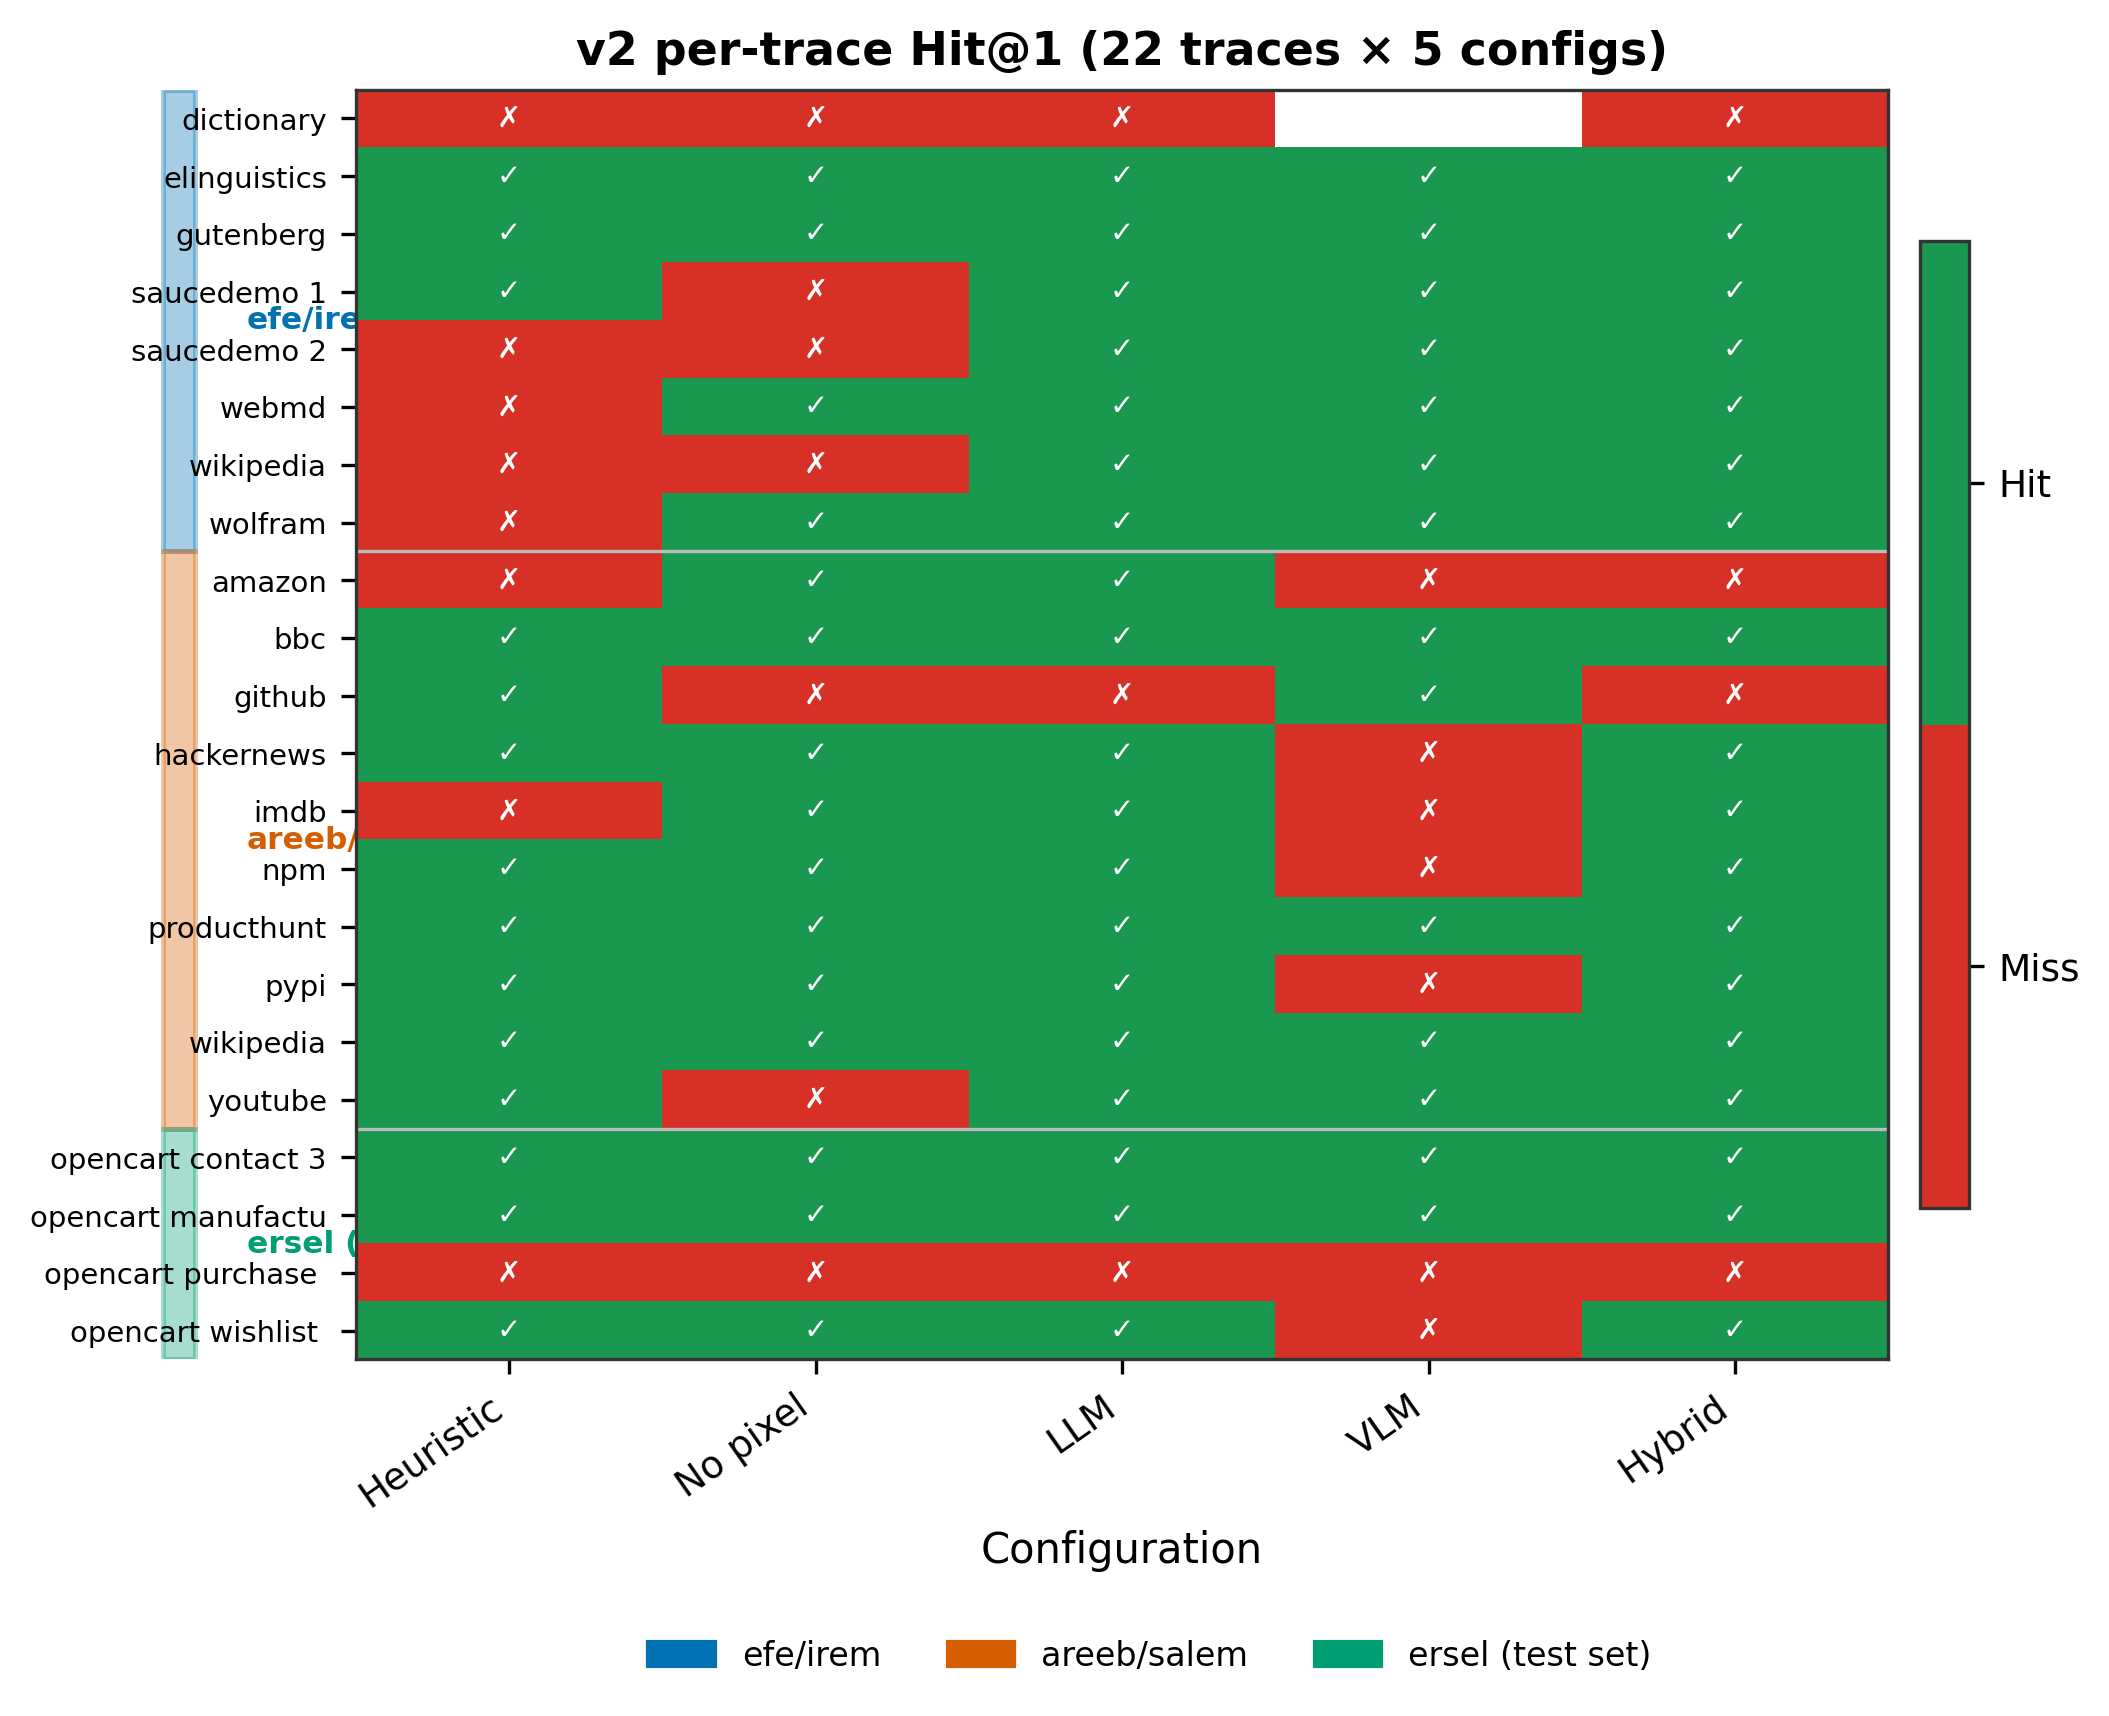
\includegraphics[width=\linewidth]{figures/fig3_v2_trace_heatmap.png}
  \caption{Per-trace Hit@1 heatmap (v2). Trace names colored by source (legend). Blank VLM cell: \texttt{dictionary} excluded (missing screenshots for top-$K$ steps).}
  \Description{Heatmap of Hit@1 per trace and mode.}
  \label{fig:heatmap}
\end{figure}

\begin{figure}[t]
  \centering
  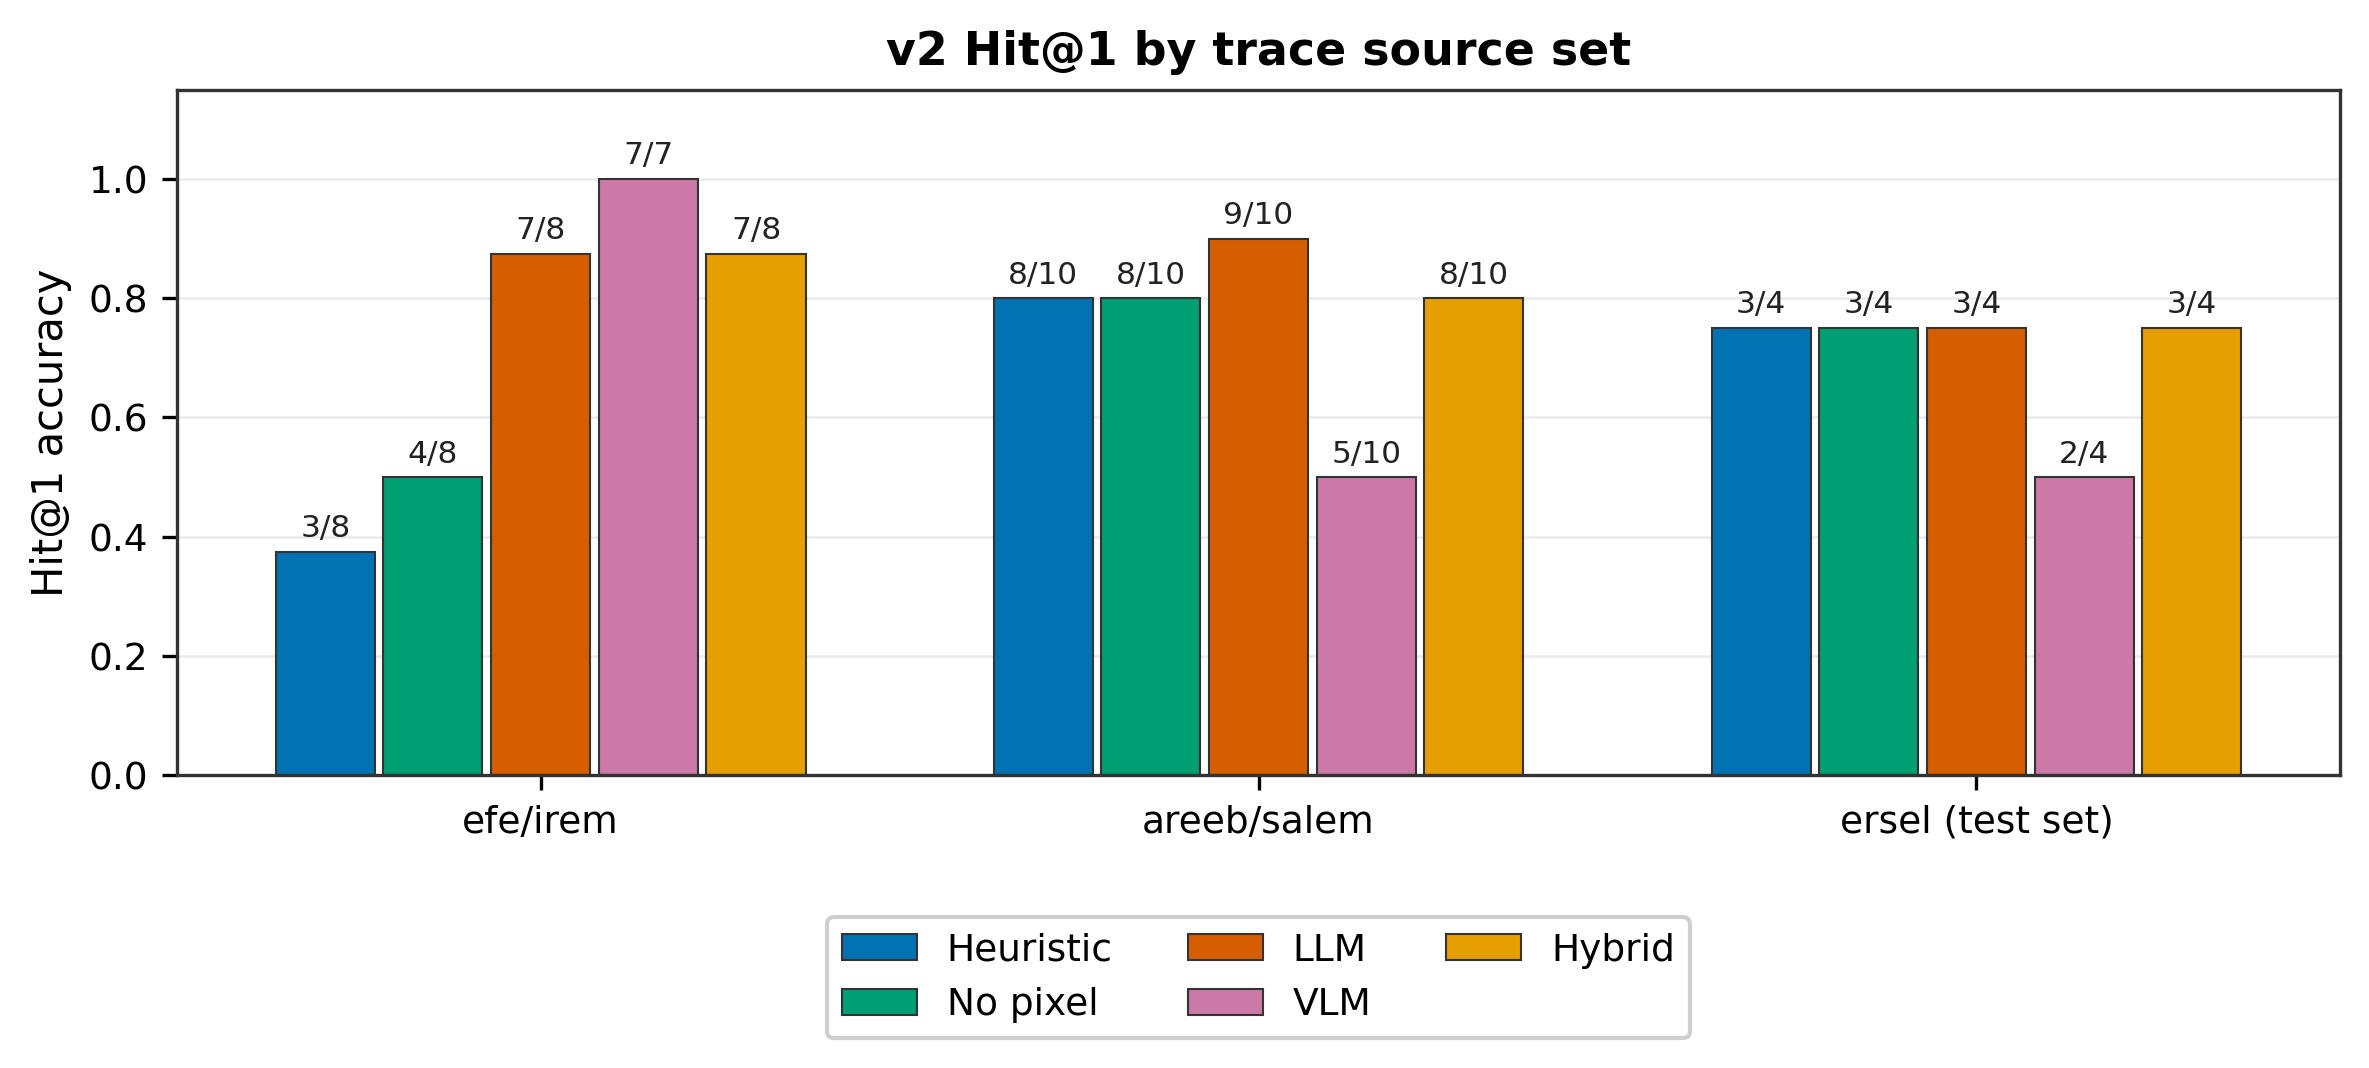
\includegraphics[width=\linewidth]{figures/fig2_v2_by_source.png}
  \caption{v2 Hit@1 by source collection and mode.}
  \Description{Bar chart of Hit@1 grouped by data source.}
  \label{fig:source}
\end{figure}

\subsection{Case studies}
\label{sec:case}

\textbf{amazon} (GT step~20, auth-gated action).
LLM ranks the causal action first (Hit@1).
Hybrid prefers an earlier scroll step with stronger pixel signal (rank distance~2).
Illustrates visual noise overriding causal text.

\textbf{github} (GT step~23, JS crash).
Both LLM and hybrid miss Hit@1, but hybrid places GT at rank~2 (distance~1) vs.\ LLM rank~5 (distance~4).
Hybrid recovers a visually evident but text-ambiguous fault in the shortlist.

\textbf{saucedemo\_2, bbc, pypi, youtube} (screenshot-primary).
The heuristic baseline misses \texttt{saucedemo\_2} (no text signal); LLM and hybrid both localize it using local visual-causal and pixel channels in v2.

\subsection{Analysis by signal type}

Grouping traces by primary signal type reveals expected mode strengths.
\textbf{Network/console faults} (9 traces): LLM reaches 89\% Hit@1 (8/9) vs.\ 67\% (6/9) for the heuristic baseline.
\textbf{Screenshot-primary faults} (4 traces): the baseline reaches 75\% Hit@1 (3/4); both LLM and hybrid reach 100\% because v2's local visual-causal scan runs even in LLM-only mode.
\textbf{Absence-of-activity} (\texttt{wolfram}, both \texttt{wikipedia} traces): navigation and missing-page features are critical; LLM reranking promotes the silent navigation fault over CDN noise.

\subsection{v1 comparison}

On partial runs, v1 heuristic reached 55\% Hit@1 ($n{=}22$); v1 hybrid ${\sim}70\%$ ($n{=}10$) did not reliably beat v1 LLM (${\sim}72\%$, $n{=}18$) due to guard interactions.
v2 hybrid on the full corpus reaches 82\% Hit@1 with 100\% Hit@3 (Table~\ref{tab:v1v2} in the appendix).

%==============================================================================
\section{Threats to Validity}
\label{sec:threats}

\textbf{Construct validity.}
Single fault-step labels simplify evaluation but blur symptom vs.\ cause (e.g., \texttt{amazon}).
Hit@$k$ and rank distance partially mitigate this by rewarding near-misses.

\textbf{Internal validity.}
Fusion weights were fixed in \texttt{v2/config.yaml} before aggregate reporting.
Structural rules were motivated by recurring failure \emph{types}, not by per-trace grid search on ground truth in v2.

\textbf{External validity.}
22 English UI traces from academic collectors are not industry-scale.
Three trace schemas limit generalization without adapter code.
Table~\ref{tab:benchmark} shows uneven fault-type coverage, so mode strengths on rare categories (e.g., JS exceptions, $n{=}1$) are estimated from small samples.

\textbf{Conclusion validity.}
LLM/VLM APIs with $T{=}0$ may still vary by provider routing; we report frozen run timestamps in the repository.
Our evaluation used \textbf{free-tier} endpoints only: Nemotron~3 Super~120B on OpenRouter for text reranking and Llama~4 Scout~17B on Groq for screenshot pairs.
Free tiers impose daily request caps, TPM throttling, and a restricted model catalog---paid alternatives (e.g., Qwen2.5-VL-72B, Gemini~2.0~Flash) may rank differently.
Because the LLM and VLM run on \emph{different} providers and model families, we do not assume equal capability across modalities; we report their complementary contributions under a fixed, cost-bounded configuration.

\textbf{Evaluation bias.}
ersel (4 traces) uses intent fields absent elsewhere.
VLM-only aggregate excludes \texttt{dictionary} ($n{=}21$): the trace artifact lacks complete pass/fail screenshot files for the heuristic top-$K$ candidates (${\sim}5$ steps), so the VLM could not analyze the ranked steps and the run is treated as unavailable (not scored as a miss).
Hybrid mode still reports a fallback ranking for \texttt{dictionary} using text and pixel channels.

%==============================================================================
\section{Conclusion}
\label{sec:conclusion}

Relative debugging of UI test regressions benefits from multimodal pass--fail comparison.
\textsc{TraceLens} demonstrates a reproducible pipeline from aligned trace diffs through LLM/VLM priors to ranked suspects and stakeholder explanations.
Against a 64\% heuristic baseline, LLM-only achieves 86\% Hit@1; hybrid fusion trades one top-1 hit for perfect Hit@3 and better rank quality.
v2's unified fusion replaces v1's trace-specific guard brittleness with a single interpretable scorer.

\textbf{Future work} includes a larger public relative-debugging benchmark, learned fusion weights, multi-fault labels, CI integration, and practitioner user studies.

%==============================================================================
\section*{Data Availability}

The repository includes trace data, ground truth, the v2 pipeline (\texttt{main2.py}), frozen metric JSONs, and figure scripts.
Regenerate figures with \texttt{python scripts/plot\_metrics.py}.

%==============================================================================
\appendix
\section{v1 Aggregate Comparison}
\label{app:v1}

\begin{table}[h]
  \caption{v1 vs.\ v2 Hit@1 on overlapping runs.}
  \label{tab:v1v2}
  \small
  \begin{tabular}{lrr}
    \toprule
    Mode & v1 Hit@1 & v2 Hit@1 \\
    \midrule
    Heuristic & 55\% ($n{=}22$) & 64\% ($n{=}22$) \\
    LLM & 72\% ($n{=}18$) & 86\% ($n{=}22$) \\
    VLM & 88\% ($n{=}17$) & 67\% ($n{=}21$) \\
    Hybrid & 70\% ($n{=}10$) & 82\% ($n{=}22$) \\
    \bottomrule
  \end{tabular}
\end{table}

v1 VLM headline accuracy on 17 traces should not be compared directly to v2 VLM on 21 traces; different coverage and fusion integration dominate.

%==============================================================================
\bibliographystyle{ACM-Reference-Format}
\bibliography{references}

\end{document}
